\subsubsection{LM2596}

El regulador conmutado reductor (o Buck converter en inglés) es un módulo que permite reducir una tensión de entrada alta a una tensión de salida menor. Esto se logra pidiendo menos corriente a la entrada y entregando más corriente a la salida.\cite{texasinstrumentsLM2596SIMPLESWITCHER}

En este caso, se utiliza para reducir la tensión de alimentación (tensión de $24 V$) a una tensión de $7 V$ para la entrada del \texttt{LDO}, que alimentará a los \texttt{INAs} y al \texttt{ESP8266}.

\begin{figure}[h]
    \centering
    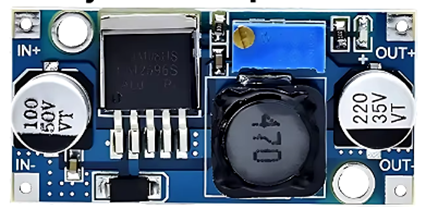
\includegraphics[width=0.5\textwidth]{images/2-hardware/componentes/LM2596.png}
    \caption{Módulo regulador reductor \texttt{LM2596}}
    \label{fig:hardware/modulos/lm2596}
\end{figure}